\documentclass[11pt]{standalone}
\usepackage{tikz}
\usetikzlibrary{shapes.geometric}
\usetikzlibrary{plotmarks}
\usetikzlibrary{arrows.meta}
\begin{document} 

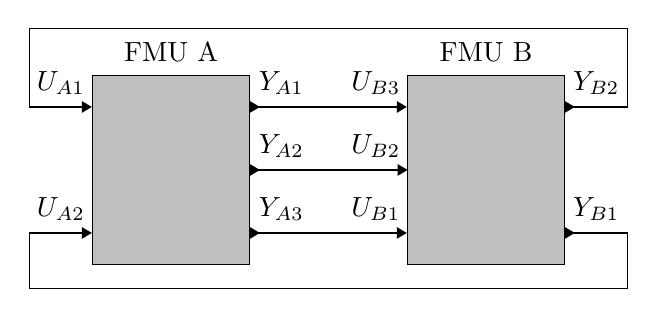
\begin{tikzpicture}
\begin{scope}
% FMU1
\node[rectangle,draw,fill=gray!50,minimum height = 2.4cm,minimum width = 2cm] (fmu1) {};

%\draw[draw=white,-{Straight Barb[angle=60:2pt 3,black]}] ([yshift=0.6cm,xshift=-0.2cm]fmu1.west) -- ([yshift=0.6cm]fmu1.west);
%\draw[draw=white,-{Straight Barb[angle=60:2pt 3,black]}] ([yshift=-0.6cm,xshift=-0.2cm]fmu1.west) -- ([yshift=-0.6cm]fmu1.west);

\node[below of=fmu1,yshift=2.5cm] {FMU A};
\node[left of=fmu1,yshift=1.1cm,xshift=-0.4cm] {$U_{A1}$};
\node[left of=fmu1,yshift=-.5cm,xshift=-0.4cm] {$U_{A2}$};
\node[right of=fmu1,yshift=1.1cm,xshift=0.4cm] {$Y_{A1}$};
\node[right of=fmu1,yshift=.3cm,xshift=0.4cm] {$Y_{A2}$};
\node[right of=fmu1,yshift=-.5cm,xshift=0.4cm] {$Y_{A3}$};

% FMU2
\node[rectangle,draw,fill=gray!50,minimum height = 2.4cm,minimum width = 2cm, xshift=4cm] (fmu2) {};

\node[below of=fmu2,yshift=2.5cm] {FMU B};
\node[left of=fmu2,yshift=1.1cm,xshift=-0.4cm] {$U_{B3}$};
\node[left of=fmu2,yshift=.3cm,xshift=-0.4cm] {$U_{B2}$};
\node[left of=fmu2,yshift=-.5cm,xshift=-0.4cm] {$U_{B1}$};
\node[right of=fmu2,yshift=1.1cm,xshift=0.4cm] {$Y_{B2}$};
\node[right of=fmu2,yshift=-.5cm,xshift=0.4cm] {$Y_{B1}$};


%Inter-FMU
\coordinate [right of =fmu2, yshift=1.8cm,xshift=.8cm] (c1);
\coordinate [left of =fmu1, yshift=1.8cm,xshift=-.8cm] (c2);

\coordinate [right of =fmu2, yshift=-1.5cm,xshift=.8cm] (c3);
\coordinate [left of =fmu1, yshift=-1.5cm,xshift=-.8cm] (c4);

\draw [-{Triangle[black]}]([yshift=.8cm]fmu2.east) -| (c1) -- (c2) |- ([yshift=.8cm]fmu1.west);
\draw [-{Triangle[black]}]([yshift=-.8cm]fmu2.east) -| (c3) -- (c4) |- ([yshift=-.8cm]fmu1.west);

\draw [-{Triangle[black]}]([yshift=-.8cm]fmu1.east) -- ([yshift=-.8cm]fmu2.west);
\draw [-{Triangle[black]}]([yshift=.8cm]fmu1.east)  -- ([yshift=.8cm]fmu2.west);

\draw[-{Triangle[black]},shorten >=-2pt] ([yshift=0.8cm]fmu1.east) -- ([yshift=0.8cm,xshift=0.05cm]fmu1.east);
\draw[-{Triangle[black]},shorten >=-2pt] ([yshift=-0.8cm]fmu1.east) -- ([yshift=-0.8cm,xshift=0.05cm]fmu1.east);
\draw[-{Triangle[black]},shorten >=-2pt] (fmu1.east) -- ([xshift=0.05cm]fmu1.east);

\draw[-{Triangle[]},shorten >=-2pt] ([yshift=0.8cm]fmu2.east) -- ([yshift=0.8cm,xshift=0.05cm]fmu2.east);
\draw[-{Triangle[]},shorten >=-2pt] ([yshift=-0.8cm]fmu2.east) -- ([yshift=-0.8cm,xshift=0.05cm]fmu2.east);

\draw[-{Triangle[]},shorten >=-2pt] (fmu1.east) -- ([xshift=-0.06cm]fmu2.west);

\end{scope}


\end{tikzpicture}

\end{document}